% 作者:Yuchen Deng〔Zz〕 QQ群:19346666、111601117
% 欢迎加群共同维护与交流

\def\publish{}
\def\all{}
% 作者:Yuchen Deng〔Zz〕 QQ群:19346666、111601117
% 欢迎加群共同维护与交流

\documentclass[a4paper,fontset=fandol,zihao=-4,linespread=1.2]{ctexbook}

% \setCJKmainfont{FandolFang-Regular.otf} %中文字体
\setmainfont[Mapping=tex-text]{PT Mono} %英文字体
\ctexset{
  chapter/format = \Large\bfseries\centering,
  section/format = \large\bfseries,
  subsection/format = \normalsize\bfseries,
  chapter/beforeskip = 0pt,
  chapter/afterskip = 3ex plus 1ex minus 0.6ex,
  section/beforeskip = 2.5ex plus 1ex minus 0.5ex,
  section/afterskip = 1.5ex plus 1ex minus 0.3ex,
  subsection/beforeskip = 2ex plus 1ex minus 0.4ex,
  subsection/afterskip = 1ex plus 0.5ex minus 0.2ex,
  today = big
}

\usepackage{geometry} %布局
\ifx\publish\undefined
\geometry{left=2.3cm,right=2.3cm,top=2.0cm,bottom=2.0cm} %页边距
\else
\geometry{left=2.6cm,right=2.0cm,top=2.0cm,bottom=2.0cm} %页边距
\fi
\setlength{\parskip}{0.2\baselineskip} %段间距
\linespread{1.1} %行间距

\usepackage[unicode=false,colorlinks,linkcolor=blue]{hyperref} %超链接
\usepackage{silence} %屏蔽警告

\usepackage{tcolorbox} %盒子
\tcbset{colback=yellow!10, colframe=red!75!black}

\usepackage{listings} %代码框
\usepackage{xunicode} %代码框星号修复
\usepackage{xcolor} %颜色

\newfontfamily\mono{Source Code Pro}
\lstset{
	columns=flexible,
	numbers=left,
	numbersep=5pt,
	frame=shadowbox,
	xleftmargin=1em,
	xrightmargin=1em,
	backgroundcolor=\color{gray!2},
	rulesepcolor=\color{gray!50},
	basicstyle=\small\mono,
	keywordstyle=\color{blue!80},
	numberstyle=\tiny\mono\color{darkgray},
	commentstyle=\it\mono\color{gray},
	stringstyle=\color[RGB]{0,168,0},
	emphstyle=\color[RGB]{166,83,0},
	showstringspaces=false,
	breaklines=true,
	language=bash,
}

\makeatletter
\lst@CCPutMacro
    \lst@ProcessOther {"2D}{-{}}
    \@empty\z@\@empty
\makeatother


\title{\kaishu {\textcolor{blue!80}{Linux\hspace{0em}技术笔记 v1.0}} \footnote{\textcolor{red!80}{本笔记所涉及到的代码或命令需结合上下文说明并理解,不能简单地复制粘贴后在终端执行。}} \ldots}
\author{\fangsong Yuchen Deng〔语晨〕{\textcolor{red!80}{\hspace{0em}「QQ\hspace{0em}群\hspace{0.2em}19346666」}}\footnote{{\textcolor{blue!80}{\hspace{0em}Linux\hspace{0.3em}技术钻研群:19346666、111601117,拥抱开源,潜心钻研Linux技术!}}}}
\date{\kaishu\today}

% \includeonly{ch01,ch03}
\begin{document}
% 作者:Yuchen Deng〔Zz〕 QQ群:19346666、111601117
% 欢迎加群共同维护与交流

\maketitle
\pagenumbering{Roman}
\tableofcontents
\newpage
\pagenumbering{arabic}
\setcounter{page}{1}
% 作者:Yuchen Deng〔Zz〕 QQ群:19346666、111601117
% 欢迎加群共同维护与交流

\ifx\all\undefined
% 作者:Yuchen Deng〔Zz〕 QQ群:19346666、111601117
% 欢迎加群共同维护与交流

\documentclass[a4paper,fontset=fandol,zihao=-4,linespread=1.2]{ctexbook}

% \setCJKmainfont{FandolFang-Regular.otf} %中文字体
\setmainfont[Mapping=tex-text]{PT Mono} %英文字体
\ctexset{
  chapter/format = \Large\bfseries\centering,
  section/format = \large\bfseries,
  subsection/format = \normalsize\bfseries,
  chapter/beforeskip = 0pt,
  chapter/afterskip = 3ex plus 1ex minus 0.6ex,
  section/beforeskip = 2.5ex plus 1ex minus 0.5ex,
  section/afterskip = 1.5ex plus 1ex minus 0.3ex,
  subsection/beforeskip = 2ex plus 1ex minus 0.4ex,
  subsection/afterskip = 1ex plus 0.5ex minus 0.2ex,
  today = big
}

\usepackage{geometry} %布局
\ifx\publish\undefined
\geometry{left=2.3cm,right=2.3cm,top=2.0cm,bottom=2.0cm} %页边距
\else
\geometry{left=2.6cm,right=2.0cm,top=2.0cm,bottom=2.0cm} %页边距
\fi
\setlength{\parskip}{0.2\baselineskip} %段间距
\linespread{1.1} %行间距

\usepackage[unicode=false,colorlinks,linkcolor=blue]{hyperref} %超链接
\usepackage{silence} %屏蔽警告

\usepackage{tcolorbox} %盒子
\tcbset{colback=yellow!10, colframe=red!75!black}

\usepackage{listings} %代码框
\usepackage{xunicode} %代码框星号修复
\usepackage{xcolor} %颜色

\newfontfamily\mono{Source Code Pro}
\lstset{
	columns=flexible,
	numbers=left,
	numbersep=5pt,
	frame=shadowbox,
	xleftmargin=1em,
	xrightmargin=1em,
	backgroundcolor=\color{gray!2},
	rulesepcolor=\color{gray!50},
	basicstyle=\small\mono,
	keywordstyle=\color{blue!80},
	numberstyle=\tiny\mono\color{darkgray},
	commentstyle=\it\mono\color{gray},
	stringstyle=\color[RGB]{0,168,0},
	emphstyle=\color[RGB]{166,83,0},
	showstringspaces=false,
	breaklines=true,
	language=bash,
}

\makeatletter
\lst@CCPutMacro
    \lst@ProcessOther {"2D}{-{}}
    \@empty\z@\@empty
\makeatother


\title{\kaishu {\textcolor{blue!80}{Linux\hspace{0em}技术笔记 v1.0}} \footnote{\textcolor{red!80}{本笔记所涉及到的代码或命令需结合上下文说明并理解,不能简单地复制粘贴后在终端执行。}} \ldots}
\author{\fangsong Yuchen Deng〔语晨〕{\textcolor{red!80}{\hspace{0em}「QQ\hspace{0em}群\hspace{0.2em}19346666」}}\footnote{{\textcolor{blue!80}{\hspace{0em}Linux\hspace{0.3em}技术钻研群:19346666、111601117,拥抱开源,潜心钻研Linux技术!}}}}
\date{\kaishu\today}

\begin{document}
% 作者:Yuchen Deng〔Zz〕 QQ群:19346666、111601117
% 欢迎加群共同维护与交流

\maketitle
\pagenumbering{Roman}
\tableofcontents
\newpage
\pagenumbering{arabic}
\setcounter{page}{1}
\fi


\setcounter{chapter}{0}

\chapter{终端基础命令}


\section{什么是终端}

\par Linux 系统安装后,绝大多数的操作都是可视化的,用鼠标和键盘与桌面交互,就可以日常使用了。但为了更好的使用或者运维 Linux 系统,我们有时还是离不开命令行的。终端就是一个通过命令来与系统交互的窗口(应用),它的英文名字叫 Terminal 。像 Ubuntu 系统、KDE Plasma 桌面,默认都绑定了 Ctrl+Alt+T 快捷键来启动终端,elementary OS 6 则默认绑定 Super+T 快捷键。没有绑定快捷键的系统,如 Debian、Fedora等,则可以通过启动器来启动,或者自己添加自定义启动快捷键。
\par 对GNOME桌面,默认的终端应用是 gnome-terminal ,KDE Plasma 桌面默认终端应用 Konsole,桌面不同,一般终端应用各异,但作用相同,用法类似。
\par 打开终端后,请依序执行以下命令,你会有收获的。
\begin{lstlisting}
    $ help
    $ whatis man
    $ man man 1
\end{lstlisting}


\ifx\all\undefined
\end{document}
\fi

% 作者:Yuchen Deng〔Zz〕 QQ群:19346666、111601117
% 欢迎加群共同维护与交流

\ifx\all\undefined
% 作者:Yuchen Deng〔Zz〕 QQ群:19346666、111601117
% 欢迎加群共同维护与交流

\documentclass[a4paper,fontset=fandol,zihao=-4,linespread=1.2]{ctexbook}

% \setCJKmainfont{FandolFang-Regular.otf} %中文字体
\setmainfont[Mapping=tex-text]{PT Mono} %英文字体
\ctexset{
  chapter/format = \Large\bfseries\centering,
  section/format = \large\bfseries,
  subsection/format = \normalsize\bfseries,
  chapter/beforeskip = 0pt,
  chapter/afterskip = 3ex plus 1ex minus 0.6ex,
  section/beforeskip = 2.5ex plus 1ex minus 0.5ex,
  section/afterskip = 1.5ex plus 1ex minus 0.3ex,
  subsection/beforeskip = 2ex plus 1ex minus 0.4ex,
  subsection/afterskip = 1ex plus 0.5ex minus 0.2ex,
  today = big
}

\usepackage{geometry} %布局
\ifx\publish\undefined
\geometry{left=2.3cm,right=2.3cm,top=2.0cm,bottom=2.0cm} %页边距
\else
\geometry{left=2.6cm,right=2.0cm,top=2.0cm,bottom=2.0cm} %页边距
\fi
\setlength{\parskip}{0.2\baselineskip} %段间距
\linespread{1.1} %行间距

\usepackage[unicode=false,colorlinks,linkcolor=blue]{hyperref} %超链接
\usepackage{silence} %屏蔽警告

\usepackage{tcolorbox} %盒子
\tcbset{colback=yellow!10, colframe=red!75!black}

\usepackage{listings} %代码框
\usepackage{xunicode} %代码框星号修复
\usepackage{xcolor} %颜色

\newfontfamily\mono{Source Code Pro}
\lstset{
	columns=flexible,
	numbers=left,
	numbersep=5pt,
	frame=shadowbox,
	xleftmargin=1em,
	xrightmargin=1em,
	backgroundcolor=\color{gray!2},
	rulesepcolor=\color{gray!50},
	basicstyle=\small\mono,
	keywordstyle=\color{blue!80},
	numberstyle=\tiny\mono\color{darkgray},
	commentstyle=\it\mono\color{gray},
	stringstyle=\color[RGB]{0,168,0},
	emphstyle=\color[RGB]{166,83,0},
	showstringspaces=false,
	breaklines=true,
	language=bash,
}

\makeatletter
\lst@CCPutMacro
    \lst@ProcessOther {"2D}{-{}}
    \@empty\z@\@empty
\makeatother


\title{\kaishu {\textcolor{blue!80}{Linux\hspace{0em}技术笔记 v1.0}} \footnote{\textcolor{red!80}{本笔记所涉及到的代码或命令需结合上下文说明并理解,不能简单地复制粘贴后在终端执行。}} \ldots}
\author{\fangsong Yuchen Deng〔语晨〕{\textcolor{red!80}{\hspace{0em}「QQ\hspace{0em}群\hspace{0.2em}19346666」}}\footnote{{\textcolor{blue!80}{\hspace{0em}Linux\hspace{0.3em}技术钻研群:19346666、111601117,拥抱开源,潜心钻研Linux技术!}}}}
\date{\kaishu\today}

\begin{document}
% 作者:Yuchen Deng〔Zz〕 QQ群:19346666、111601117
% 欢迎加群共同维护与交流

\maketitle
\pagenumbering{Roman}
\tableofcontents
\newpage
\pagenumbering{arabic}
\setcounter{page}{1}
\fi

\setcounter{chapter}{1}

\chapter{软件包管理}



\ifx\all\undefined
\end{document}
\fi

% 作者:Yuchen Deng〔Zz〕 QQ群:19346666、111601117
% 欢迎加群共同维护与交流

\ifx\all\undefined
% 作者:Yuchen Deng〔Zz〕 QQ群:19346666、111601117
% 欢迎加群共同维护与交流

\documentclass[a4paper,fontset=fandol,zihao=-4,linespread=1.2]{ctexbook}

% \setCJKmainfont{FandolFang-Regular.otf} %中文字体
\setmainfont[Mapping=tex-text]{PT Mono} %英文字体
\ctexset{
  chapter/format = \Large\bfseries\centering,
  section/format = \large\bfseries,
  subsection/format = \normalsize\bfseries,
  chapter/beforeskip = 0pt,
  chapter/afterskip = 3ex plus 1ex minus 0.6ex,
  section/beforeskip = 2.5ex plus 1ex minus 0.5ex,
  section/afterskip = 1.5ex plus 1ex minus 0.3ex,
  subsection/beforeskip = 2ex plus 1ex minus 0.4ex,
  subsection/afterskip = 1ex plus 0.5ex minus 0.2ex,
  today = big
}

\usepackage{geometry} %布局
\ifx\publish\undefined
\geometry{left=2.3cm,right=2.3cm,top=2.0cm,bottom=2.0cm} %页边距
\else
\geometry{left=2.6cm,right=2.0cm,top=2.0cm,bottom=2.0cm} %页边距
\fi
\setlength{\parskip}{0.2\baselineskip} %段间距
\linespread{1.1} %行间距

\usepackage[unicode=false,colorlinks,linkcolor=blue]{hyperref} %超链接
\usepackage{silence} %屏蔽警告

\usepackage{tcolorbox} %盒子
\tcbset{colback=yellow!10, colframe=red!75!black}

\usepackage{listings} %代码框
\usepackage{xunicode} %代码框星号修复
\usepackage{xcolor} %颜色

\newfontfamily\mono{Source Code Pro}
\lstset{
	columns=flexible,
	numbers=left,
	numbersep=5pt,
	frame=shadowbox,
	xleftmargin=1em,
	xrightmargin=1em,
	backgroundcolor=\color{gray!2},
	rulesepcolor=\color{gray!50},
	basicstyle=\small\mono,
	keywordstyle=\color{blue!80},
	numberstyle=\tiny\mono\color{darkgray},
	commentstyle=\it\mono\color{gray},
	stringstyle=\color[RGB]{0,168,0},
	emphstyle=\color[RGB]{166,83,0},
	showstringspaces=false,
	breaklines=true,
	language=bash,
}

\makeatletter
\lst@CCPutMacro
    \lst@ProcessOther {"2D}{-{}}
    \@empty\z@\@empty
\makeatother


\title{\kaishu {\textcolor{blue!80}{Linux\hspace{0em}技术笔记 v1.0}} \footnote{\textcolor{red!80}{本笔记所涉及到的代码或命令需结合上下文说明并理解,不能简单地复制粘贴后在终端执行。}} \ldots}
\author{\fangsong Yuchen Deng〔语晨〕{\textcolor{red!80}{\hspace{0em}「QQ\hspace{0em}群\hspace{0.2em}19346666」}}\footnote{{\textcolor{blue!80}{\hspace{0em}Linux\hspace{0.3em}技术钻研群:19346666、111601117,拥抱开源,潜心钻研Linux技术!}}}}
\date{\kaishu\today}

\begin{document}
% 作者:Yuchen Deng〔Zz〕 QQ群:19346666、111601117
% 欢迎加群共同维护与交流

\maketitle
\pagenumbering{Roman}
\tableofcontents
\newpage
\pagenumbering{arabic}
\setcounter{page}{1}
\fi


\setcounter{chapter}{2}

\chapter{系统维护}


\section{查看开机启动时间}

\par Linux 系统可以自由的查看开机服务所占用的时间,如果发现启动速度变慢,或者进入桌面后要等待几秒才正常显示,则可以执行下面的命令:
\begin{lstlisting} [numbers=none]
    $ systemd-analyze critical-chain
\end{lstlisting}
\par 执行效果图如图 \ref{fig:2021-10-28_09-55-54} 所示。

\begin{figure} [htbp]
	\centering
	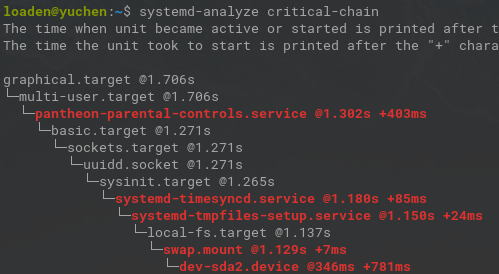
\includegraphics [width=0.8\textwidth]{images/ch03/2021-10-28_09-55-54.png}
	\caption{查看桌面启动时间}
	\label{fig:2021-10-28_09-55-54}
\end{figure}

\par 此外,下面的命令可选择输出启动过程详细信息或简要信息,可供维护参考。
\begin{lstlisting}
    $ systemd-analyze blame
    $ systemd-analyze
\end{lstlisting}


\ifx\all\undefined
\end{document}
\fi

\end{document}



\begin{lstlisting}
\end{lstlisting}

\begin{lstlisting} [numbers=none]
\end{lstlisting}

\begin{lstlisting} [firstnumber=12]
\end{lstlisting}


\begin{enumerate}
	\item 序号1
	\item 序号2
\end{enumerate}


{\vspace{10pt}}
\begin{tcolorbox}[title=标题]
	\par{\bf{分隔线}}
	\tcblower
	\par{\bf{段落1}}
	\par{\bf{段落2}}
\end{tcolorbox}


{\bf{粗体}}
{\mono{'*'}}
\footnote{脚注}
$\backslash$ %\∼
$\sim$ %∼


% 图片使用示例1:绽放图片宽度至文字宽度的96%
\begin{figure} [htbp]
	\centering
	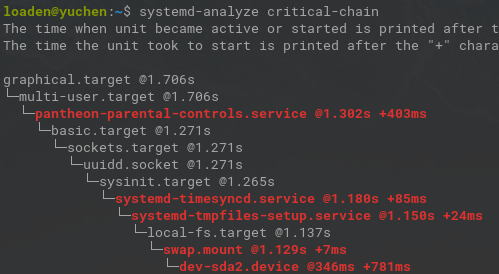
\includegraphics [width=0.96\textwidth]{images/ch03/2021-10-28_09-55-54.png}
	\caption{查看桌面启动时间}
	\label{fig:2021-10-28_09-55-54}
\end{figure}

% 图片使用示例2:绽放图片至自身宽度的90%
\begin{figure} [htbp]
	\centering
	\includegraphics [scale=0.9]{images/ch03/2021-10-28 09-55-54.png}
	\caption{查看桌面启动时间}
	\label{fig:2021-10-28_09-55-54}
\end{figure}

% 引用图片
\par 如图 \ref{fig:2021-10-28 09-55-54} 所示


% 并排图片
\begin{figure}[H]
	\centering
	\begin{minipage}{0.48\textwidth}
		\centering
		\includegraphics{pic1.png}
		\caption{Title of pic1}
	\end{minipage}
	\begin{minipage}{0.48\textwidth}
		\centering
		\includegraphics{pin2.png}
		\caption{Title of pic2}
	\end{minipage}
\end{figure}


% 环绕图片,position可以有r或者l两种选项
\begin{wrapfigure}{position}{width}
	\centering
	\includegraphics{pic.png}
\end{wrapfigure}
